\chapter{\IfLanguageName{dutch}{Stand van zaken}{State of the art}}%
\label{ch:stand-van-zaken}

% Tip: Begin elk hoofdstuk met een paragraaf inleiding die beschrijft hoe
% dit hoofdstuk past binnen het geheel van de bachelorproef. Geef in het
% bijzonder aan wat de link is met het vorige en volgende hoofdstuk.

% Pas na deze inleidende paragraaf komt de eerste sectiehoofding.

De Securities and Exchange Commission (SEC) vereist dat institutionele vermogensbeheerders een kwartaalrapport indienen dat bekend staat als Form 13F als ze zeggenschap hebben over \$100 miljoen of meer in sectie 13(f) effecten. Sectie 13(f) van de Securities Exchange Act van 1934 verplicht de openbaarmaking van effectenbezit door grote institutionele beleggers om de transparantie te vergroten. In 1975 implementeerde het Congres deze bepaling om de toegankelijkheid van informatie over de investeringsactiviteiten van deze bedrijven te verbeteren. De bedoeling was om het vertrouwen van beleggers in de integriteit van de effectenmarkten in de Verenigde Staten te vergroten door middel van een openbaarmakingsprogramma \textcite{SECform13F2024}.
Melding 13F biedt een uitgebreid overzicht van de aandelenbeleggingen van S\&P 500 bedrijven en is een zeer belangrijk hulpmiddel voor analisten, onderzoekers en beleggers die inzicht willen verkrijgen in markttrends en de beleggingsbenaderingen van belangrijke marktspelers. Het onverwerkte tekstformaat waarin deze inzendingen worden aangeleverd, vormt echter een aanzienlijke belemmering voor effectieve gegevensextractie en -analyse, vooral voor inzendingen van voor 2013. Voor 2013 ontbrak het bij 13F-meldingen vaak aan standaardisatie en systematische opmaak, wat nu wel gebruikelijk is bij recentere aanmeldingen.
Kunstmatige intelligentie (AI) en Machine Learning (ML) technologieën hebben de extractie en organisatie van gegevens uit ongestructureerde tekst de afgelopen jaren aanzienlijk veranderd. Geavanceerde methodologieën zoals Natural Language Processing (NLP) en Deep Learning (DL) modellen vergemakkelijken de omzetting van tekstuele 13F meldingen in gestructureerde datasets die geschikt zijn voor grondige analyse en studie. Standaardisatie is cruciaal voor historische gegevens, omdat het ontbreken van uniformiteit geautomatiseerde verwerking kan bemoeilijken. Door gebruik te maken van deze technologieën kunnen we zowel huidige als oudere 13F aanvragen omzetten in georganiseerde gegevens, die vervolgens kunnen worden opgeslagen in databanken, waardoor patronen eenvoudiger kunnen worden opgehaald, gevisualiseerd en geanalyseerd.
\\

Het doel van deze literatuurstudie is het onderzoeken en beoordelen van de verschillende Artificial Intelligence (AI) en Machine Learning (ML) technieken die kunnen worden gebruikt om gegevens uit 13F-meldingen van voor 2013 te extraheren, te organiseren en op te slaan. Het doel van het onderzoek is het bepalen van de meest efficiënte methoden om de ongeorganiseerde inhoud van deze documenten om te zetten in een gestructureerd formaat dat geschikt is voor analyse en opslag in een database. Dit houdt in dat er een onderzoek wordt gedaan naar verschillende kunstmatige intelligentie methodologieën, zoals Natural Language Processing (NLP) en Text mining, en dat bepaalde tools zoals NLTK en SpaCy worden geëvalueerd. De literatuurstudie zal ook de integratie van gestructureerde gegevens in een Database Management System (DBMS) onderzoeken, om te garanderen dat de geëxtraheerde gegevens gemakkelijk beschikbaar zijn voor later onderzoek en analyse. Het doel van deze evaluatie is om een uitgebreide kennis te krijgen van de meest effectieve procedures en technologie voor het verwerken van 13F-meldingen. 

% ----------------------------------------------------------------------------
\section{Wat zijn 13F meldingen}

Het doel van deze sectie is om een beknopte inleiding te geven aan 13F-meldingen, met bijzondere aandacht voor de structuur van deze meldingen, de informatie die ze bevatten en de reden van hun bestaan.


\subsection{Definitie en doel}
Volgens \autocite{SECform13F2024} zijn 13F-meldingen verplichte wettelijke documenten die de Amerikaanse Securities and Exchange Commission (SEC) vereist onder Sectie 13(f) van de Securities Exchange Act van 1934. Deze deponeringen worden gebruikt om de portefeuilles van institutionele beleggingsbeheerders te rapporteren.

Het belangrijkste doel van 13F meldingen is om duidelijkheid en openheid te bieden over de beleggingsactiviteiten van belangrijke institutionele beleggers. Deze vereiste vergemakkelijkt het toezicht op beleggingsposities van verschillende instellingen, zoals beleggingsfondsen, pensioenfondsen en andere belangrijke beleggingsbeheerders, door het publiek en regelgevende instanties.

\subsection{Belangrijke kenmerken}
Het doel van dit deel is het bespreken van enkele kenmerken van de 13F-meldigen waaronder wie het moet indienen en wat ze moeten inhouden.


\subsubsection{Vereisten voor rapportage:}

Institutionele beleggingsbeheerders die minimaal \$100 miljoen aan beheerd vermogen beheren, zijn verplicht om elk kwartaal een 13F-melding in te dienen. Deze rapporten moeten gedetailleerde informatie bevatten over de aandelenportefeuille van de instelling. Dit omvat onder andere de naam van het aandeel, het CUSIP-nummer, het aantal aandelen dat wordt gehouden, en de marktwaarde ervan. 

\subsubsection{Omvang van de informatie:}

De rapportages over het aandelenbezit van grote beleggingsinstellingen richten zich voornamelijk op aandelen, terwijl andere soorten activa, zoals obligaties, derivaten en private equity, buiten beschouwing worden gelaten. Elk kwartaalrapport biedt een beknopt overzicht van de aandelenportefeuille van de instelling aan het einde van de rapportageperiode. Dit overzicht geeft waardevolle inzichten in de investeringsstrategieën en methoden die de instelling hanteert, wat bijdraagt aan de transparantie en begrip van hun beleggingsbenadering.


\subsubsection{Opmaak en toegankelijkheid:}
De 13F-meldingen van voor 2013 zijn varierend in opmaak, dit is wat data extractie moeilijk maakt
Dit zijn enkele afbeeldingen van enkele van de tienduizenden 13F-meldingen

\paragraph{Voor 2013}
Hier ziet men een aantal voorbeelden van informatie tabel van enkele 13F meldigen. Zoals men ziet zijn er veel verschillende manieren waarop deze meldingen zijn ingediend.
\begin{figure}[hbt!]
     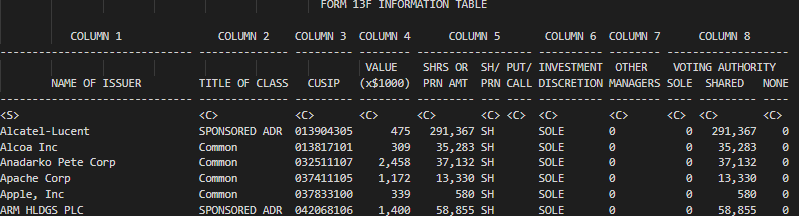
\includegraphics[width=0.8\textwidth]{13F_EX0.png}
     \caption[13F voorbeeld 1]{\label{fig:voorbeeld 1}Een correcte 13F melding duidelijk gestructureerd en geen missende waarden}
\end{figure}


\begin{figure}[hbt!]
    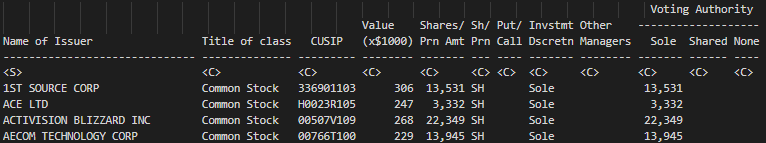
\includegraphics[width=0.8\textwidth]{13F_EX2.png}
    \caption[13F voorbeeld 3]{\label{fig:voorbeeld 2}Een 13F melding met missende waarden}
\end{figure}
\begin{figure}[hbt!]
    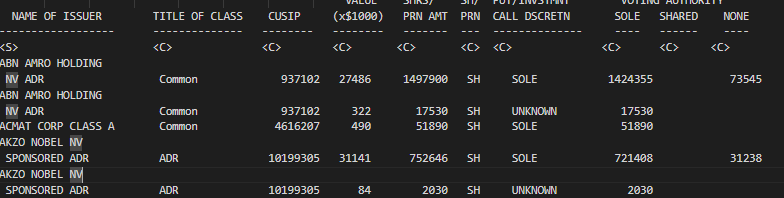
\includegraphics[width=0.8\textwidth]{13F_EX3.png}
    \caption[13F voorbeeld 4]{\label{fig:voorbeeld 3}Een 13F melding met missende waarden en één entry overspant minstens één rij}
\end{figure}

\begin{figure}[hbt!]
    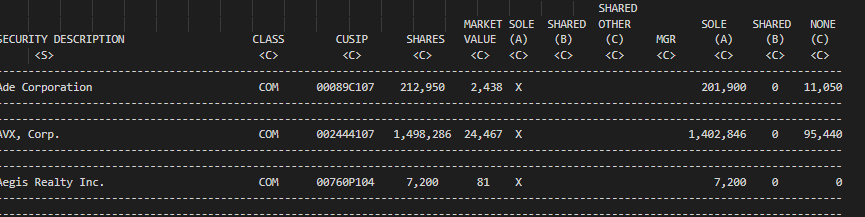
\includegraphics[width=0.8\textwidth]{13F_EX4.png}
    \caption[13F voorbeeld 5]{\label{fig:voorbeeld 4}Een 13F melding gebruik makend van `X` in plaats van Bv. Sole}
\end{figure}

\begin{figure}[hbt!]
    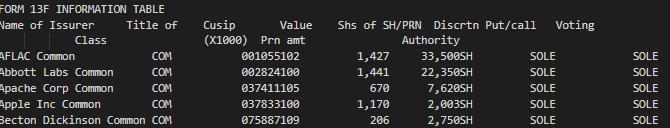
\includegraphics[width=0.8\textwidth]{13F_EX5.png}
    \caption[13F voorbeeld 6]{\label{fig:voorbeeld 5}Een 13F melding zonder cijfer datas in de laatste kolommen}
\end{figure}

\begin{figure}[hbt!]
    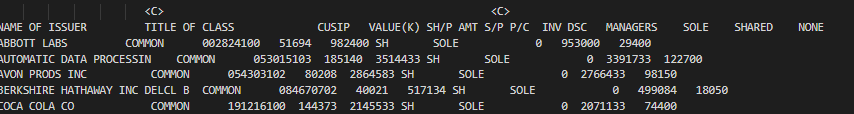
\includegraphics[width=0.8\textwidth]{13F_EX6.png}
    \caption[13F voorbeeld 7]{\label{fig:voorbeeld 6}Een 13F melding zonder gestructureerde data maar werkend met tabs, geen tabel structuur}
\end{figure}
\paragraph{Na 2013}

\begin{figure}[hbt!]
    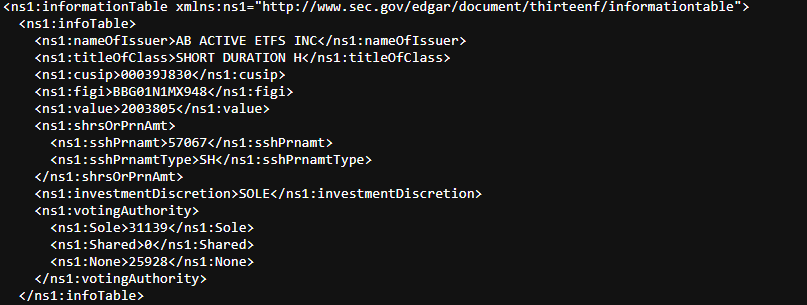
\includegraphics[width=0.8\textwidth]{13F_24_EX1.png}
    \caption[13F voorbeeld 7]{\label{fig:voorbeeld 2024 1}Een recente (2024) 13F melding gestructureerd in XML}
\end{figure}
% ----------------------------------------------------------------------------


\section{Text mining en gerelateerde technieken}
Text mining, of ook bekend tekstdatamining, is de procedure om ongestructureerde tekst om te zetten in een gestructureerd formaat om significante patronen te ontdekken en nieuwe inzichten te verwerven. Text mining maakt de analyse van uitgebreide tekstdatasets mogelijk om significante thema's, patronen en verborgen verbanden bloot te leggen. Deze techniek is essentieel voor het omzetten van ongestructureerde gegevens in gestructureerde gegevens, die vervolgens kunnen worden gebruikt voor analyse en besluitvorming\autocite{IBM2024}.

\subsection{Document datatypes}
Text mining kan verschillende soorten gegevens omvatten, waaronder:

\begin{itemize}
  \item \textbf{Gestructureerde Gegevens}: Deze gegevens zijn gestandaardiseerd in een tabelvorm, wat ze makkelijker maakt om op te slaan en te verwerken voor analyse en machine learning-algoritmen. Voorbeelden includeren databanken met kolommen en rijen.
  \item \textbf{Ongestructureerde Gegevens}: Deze gegevens hebben geen vooraf gedefinieerd formaat en kunnen tekst uit bronnen zoals sociale media of productrecensies bevatten, evenals rijke media zoals video- en audiobestanden. Aangezien financiële documenten vaak in ongestructureerd formaat bestaan, is text mining essentieel om deze gegevens om te zetten in een bruikbaar formaat.
  \item \textbf{Semi-gestructureerde Gegevens}: Deze gegevens vormen een mix tussen gestructureerde en ongestructureerde formaten. Ze hebben enige organisatie, maar voldoen niet volledig aan de vereisten van een relationele database. Voorbeelden hiervan zijn XML, JSON en Html-bestanden.
\end{itemize}

Dit onderscheid zijn van groot belang voor het begrijpen van hoe text mining toegepast kan worden over de verschillende datastructuren, dit opent de mogelijkheid om de data de extraheren en belangrijke inzichten te verwerven\autocite{AWS2024}.

\subsection{Text mining vs. Text analytics}
Hoewel text mining en text analytics vaak door elkaar worden gebruikt, kan er een genuanceerd onderscheid tussen de twee gemaakt worden. Bij text mining gaat het meestal om het identificeren van patronen en trends in ongestructureerde gegevens, terwijl text analytics gericht is op het afleiden van kwantitatieve inzichten door gegevens op een gestructureerde manier te analyseren. Deze observaties kunnen vervolgens grafisch worden weergegeven om de ontdekkingen effectief over te brengen aan een breder publiek.\autocite{IBM2024}
\subsubsection{Text mining: vinden van verstopte patronen}
Text mining omvat het extraheren van waardevolle informatie en het identificeren van verborgen patronen uit uitgebreide verzamelingen ongeorganiseerde of gedeeltelijk georganiseerde tekstuele gegevens. Text mining is een gespecialiseerde vorm van datamining die is ontworpen om vooral tekstuele informatie te verwerken. Het belangrijkste doel van text mining is om tekst om te zetten in analyseerbare gegevens om inzichten, trends en patronen te ontdekken die niet direct voor de hand liggen. Deze aanpak omvat een reeks methodologieën, waaronder het ophalen van informatie, natuurlijke taalverwerking (NLP) en machinaal leren. Het primaire doel is het begrijpen en analyseren van uitgebreide tekstdatabases \autocite{gaikwad2014text}.

\paragraph{Voor- en nadelen text mining}
Volgens \autocite{Kinter2024} en \autocite{gaikwad2014text} zijn er veel voor- en nadelen aan text mining:
\begin{itemize}
    \item Voordelen:
  \begin{itemize}
    \item Het corpus van teksten kan worden geanalyseerd met technieken zoals informatie-extractie om de namen van verschillende entiteiten en hun relaties te identificeren. 
    \item De complexe taak om effectief om te gaan met grote hoeveelheden ongestructureerde gegevens om patronen bloot te leggen, wordt aangepakt door het gebruik van text mining.
    \item Bedrijven kunnen een uitgebreid inzicht krijgen in huidige trends en patronen door inzichten te analyseren die zijn verkregen uit vele gegevensbronnen. Deze inzichten helpen bedrijven bij het nemen van weloverwogen zakelijke beslissingen.

  \end{itemize}
  \item Nadelen
  \begin{itemize}
    \item Text mining gebruikt vaak een grote hoeveelheid gegevens. Het efficiënt opslaan, beheren en verwerken van deze gegevens vereist daarom een grote hoeveelheid opslagruimte en rekenkracht, wat duur kan zijn.
    \item Text mining, gegevensanalyse en patroonherkenning zijn sterk afhankelijk van de kwaliteit van de gegevens. De nauwkeurigheid van de resultaten kan worden beïnvloed door variaties in de gegevenskwaliteit, die worden beïnvloed door de structuur en voorbewerking van de gegevens.
  \end{itemize}
\end{itemize}

\subsubsection{Text analyse: het afleiden van semantische betekenis}
Tekstanalyse daarentegen houdt zich meer bezig met het begrijpen en interpreteren van de inhoud van tekst om er informatie van hoge kwaliteit uit af te leiden. In tegenstelling tot text mining, dat zich richt op het ontdekken van nieuwe patronen, is tekstanalyse gericht op het extraheren en interpreteren van bestaande informatie uit tekstgegevens. Dit proces omvat de toepassing van semantische analysetechnieken om de betekenis, context en bedoeling achter de woorden in de tekst te begrijpen \autocite{gaikwad2014text}.

Tekstanalyse maakt vaak gebruik van Natural Language Processing (NLP) om de structuur van zinnen te ontleden, entiteiten te identificeren en sentiment te analyseren. Deze technieken zijn cruciaal voor taken zoals sentimentanalyse, waarbij het doel is om de emotionele toon van een tekst te bepalen, of onderwerpmodellering, waarbij het doel is om de belangrijkste thema's te identificeren die in een set documenten worden besproken. Tekstanalyse kan ook meer geavanceerde methoden omvatten, zoals entiteitherkenning, waarbij belangrijke stukken informatie (zoals namen, data en locaties) in een tekst worden geïdentificeerd en geclassificeerd.

\paragraph{conclusie}
Terwijl text mining vaak verkennend is, waarbij gezocht wordt naar onbekende patronen, is tekstanalyse gerichter, waarbij de nadruk ligt op het extraheren van specifieke informatie van hoge kwaliteit uit de tekst. In een juridische context kan tekstanalyse bijvoorbeeld worden gebruikt om relevante clausules uit een contract te halen, terwijl text mining kan worden gebruikt om trends in juridische beslissingen in de loop van de tijd te identificeren \autocite{gaikwad2014text}.

\subsection{Text mining technieken}
\autocite{Talib2016TextMining} spreekt over enkele technieken zoals Information Extraction (IE), Information retrieval (IR), en Meerdere NLP technieken die gebruikt worden in data mining, deze zullen hier besproken worden

\subsubsection{Information retrieval vs Information extraction}
\paragraph{Information retrieval}
Informatie retrieval (Information Retrieval, IR) verwijst naar de interactie tussen mens en computer wanneer een gebruiker informatie zoekt die overeenkomt met zijn of haar zoekopdracht in een database of computersysteem. Dit proces omvat het ophalen van relevante inhoud op basis van de behoeften van de gebruiker. Het systeem vergelijkt de zoekopdracht van de gebruiker met een reeks documenten om de meest relevante te identificeren en presenteert deze uiteindelijk in een geprioriteerde lijst. Dit gespecialiseerde vakgebied, zoals beschreven door Krallinger (2024), is essentieel om gebruikers in staat te stellen snel en efficiënt informatie te lokaliseren en extraheren uit uitgebreide en vaak ongestructureerde gegevensbronnen zoals tekstdocumenten, databases of het internet.

De effectiviteit van een IR-systeem wordt gemeten aan de hand van metrieken zoals precisie en recall. Precisie is de verhouding tussen het aantal relevante documenten dat wordt opgehaald en het totale aantal opgehaalde documenten, terwijl recall de verhouding is tussen het aantal relevante documenten dat wordt opgehaald en het totale aantal relevante documenten in de dataset \autocite{Javija2024}. Deze metrics helpen om informatie-overload te verminderen door ervoor te zorgen dat alleen de meest relevante informatie aan de gebruiker wordt gepresenteerd. De methoden en technieken die worden gebruikt in IR-systemen zijn fundamenteel voor het aandrijven van technologieën zoals zoekmachines, die een snelle en efficiënte informatie ophaling mogelijk maken \autocite{Krallinger2024}.

Enkele IR technieken zijn maar niet gelimiteerd tot \autocite{IBM2024}:
\begin{itemize}
  \item Tokenizatie: Dit is het proces van het opbreken van text in zinnen en woorden genoemd tokens. Deze zijn dan gebruikt in de modellen voor clustering en documentmatching taken\autocite{IBM2024}.
  \item Stemming is een tekstvoorbewerkingsmethode die wordt gebruikt in natuurlijke taalverwerking (NLP) om woorden te vereenvoudigen door ze om te zetten naar hun basisvorm. Het doel van stemming is om woorden te stroomlijnen en te normaliseren en zo de efficiëntie van het ophalen van informatie, het categoriseren van teksten en andere natuurlijke taalverwerkingsactiviteiten (NLP) te verbeteren\autocite{SC2024}.
\end{itemize}

\paragraph{Information Extraction}
Informatie-extractie (IE) is gericht op het extraheren van gestructureerde informatie uit ongestructureerde documenten met behulp van technieken zoals Natural Language Processing (NLP). In tegenstelling tot Information Retrieval (IR), waarbij relevante documenten worden opgehaald, richt IE zich op het identificeren van specifieke gegevens binnen deze teksten, waardoor informatie toegankelijker en analyseerbaarder wordt \autocite{Javija2024}. IE-systemen moeten kosteneffectief en aanpasbaar zijn en in staat zijn om zich over verschillende domeinen uit te breiden. Op gebieden zoals financiën wordt Named-Entity Recognition (NER) gebruikt om vooraf gedefinieerde gegevenstypen, zoals namen en data, uit documenten te extraheren, wat efficiënt gegevensbeheer vergemakkelijkt \autocite{Gupta2020}. Geautomatiseerd leren in IE vermindert fouten en afhankelijkheid van handmatig toezicht, waardoor het proces efficiënter en contextueel waardevoller wordt. De toenemende hoeveelheid ongestructureerde gegevens, vooral online, benadrukt het belang van effectieve IE-systemen \autocite{Javija2024}.


Enkele IE technieken zijn maar niet gelimiteerd tot \autocite{IBM2024}:
\begin{itemize}
  \item Feature selection en Feature extraction
  \begin{itemize}
    \item Feature selection: is een essentiële stap bij het verwerken van gegevens met een groot aantal dimensies. Het gaat om het kiezen van een kleinere set belangrijke kenmerken uit de originele set om de efficiëntie en nauwkeurigheid van het leren te verbeteren. Door overbodige en inconsequente kenmerken te elimineren, wordt de omvang van de gegevensverwerking verkleind, wordt de tijd die nodig is voor het leren verminderd en worden de resultaten gestroomlijnd. Eigenschapsselectie is een proces dat de belangrijkste oorspronkelijke kenmerken behoudt, in tegenstelling tot kenmerkextractie waarbij gegevens worden veranderd in kenmerken die goed zijn in het herkennen van patronen. Eigenschapsselectie is cruciaal voor het verminderen van de dimensionaliteit van gegevens. Technieken voor kenmerkselectie omvatten een reeks benaderingen, zoals supervised, unsupervised en semi-supervised modellen. Deze methoden worden geclassificeerd op basis van hun associatie met leermethoden (filter, wrapper, inbeddingsmodellen) en andere criteria. Eigenschapsselectie is een veelgebruikte techniek in gebieden zoals beeldherkenning en tekst mining. Het verbetert de prestaties van modellen voor machinaal leren door een evenwicht te bereiken tussen hoge nauwkeurigheid en lage rekenvereisten \autocite{CAI201870}.
    \item Feature extraction: is een essentiële stap in machinaal leren, omdat het uitgebreide invoergegevens omzet in een beter hanteerbare en lager-dimensionale kenmerkenset. Deze procedure vereenvoudigt de gegevens door de complexiteit ervan te verminderen, terwijl belangrijke informatie toch behouden blijft. Het is vooral nuttig bij taken zoals categorisatie. Kenmerkextractietechnieken transformeren de initiële kenmerkruimte in een gecondenseerde, alternatieve ruimte door een gereduceerde, representatieve verzameling kenmerken te behouden in plaats van ze weg te gooien. Principale Componenten Analyse (PCA) en Bag of Words zijn vaak gebruikte technieken. PCA vermindert bijvoorbeeld de dimensionaliteit van gegevens door de oorspronkelijke variabelen om te zetten in ongecorrigeerde componenten. Dit proces verbetert de rekenefficiëntie en verhoogt de nauwkeurigheid van modellen voor machinaal leren \autocite{Mustazzihim}.
    \item Verschil? FS behoud de originele features terwijl FE nieuwe maakt.
  \end{itemize}
    \item  Named Entity Recognition (NER) is een kerntaak in Natural Language Processing (NLP) die tot doel heeft entiteiten, zoals personen, organisaties en plaatsen, binnen een gegeven tekst te herkennen en te categoriseren. NER, of Named Entity Recognition, wordt op grote schaal gebruikt in een verscheidenheid aan toepassingen, variërend van het ophalen van informatie tot geautomatiseerde klantenservice.
    


    Recent onderzoek benadrukt dat, hoewel NER-modellen opmerkelijke prestaties hebben behaald op typische datasets en vaak hoge F-scores laten zien, deze maat alleen geen goed inzicht geeft in hun effectiviteit. Geavanceerde NER-modellen vertonen bijvoorbeeld F-scores van meer dan 90\% op datasets zoals OntoNotes. Desalniettemin kan deze eenzame metriek variaties in prestaties verdoezelen tussen verschillende categorieën entiteiten, soorten taal en onbekende data \autocite{vajjala2022reallyknowstateart}.
    
\end{itemize}


\begin{table}[h!]
  \centering
  \begin{tabular}{|p{4cm}|p{5cm}|p{5cm}|}
  \hline
  \textbf{Aspect} & \textbf{Information Retrieval} & \textbf{Information Extraction} \\ \hline
  \textbf{Focus} & Document Retrieval & Feature Retrieval \\ \hline
  \textbf{Uitvoer} & Geeft een set van documenten terug & Geeft feiten van een document terug \\ \hline
  \textbf{Doel} & Het doel is om documenten te vinden die relevant zijn voor de informatiebehoefte van de gebruiker. & Het doel is om vooraf gespecificeerde kenmerken uit documenten te halen of informatie weer te geven. \\ \hline
  \textbf{Aard van informatie} & Echte informatie ligt verborgen in documenten & Extraheer informatie uit de documenten \\ \hline
  \textbf{Application} & Used in many search engines – Google is the best IR system for the web. & Used in database systems to enter extracted features automatically. \\ \hline
  \textbf{Methodology} & Typically uses a bag of words model of the source text. & Typically based on some form of semantic analysis of the source text. \\ \hline
  \textbf{Theoretical Basis} & Mostly use the theory of information, probability, and statistics. & Emerged from research into rule-based systems. \\ \hline
  \end{tabular}
  \caption{Comparison of Information Retrieval and Information Extraction}
  \label{tab:ir_vs_ie}
  \end{table}
  
 \paragraph{Conclusie}
 Information Retrieval (IR) en Information Extraction (IE) zijn twee technologieën die informatie toegankelijk maken via verschillende methodologieën.IR richt zich op het ophalen van relevante documenten, terwijl IE specifieke, gestructureerde informatie extraheert voor nauwkeurige gegevensanalyse.IR is essentieel voor grote datasets en zoekmachines, terwijl IE cruciaal is voor het extraheren van bruikbare inzichten. De kracht van IR ligt in het beheren en ophalen van informatie uit ongestructureerde bronnen, waardoor het onmisbaar is voor grote databases. IE is van vitaal belang voor datamining, kennisbeheer en geautomatiseerde processen. Naarmate het datavolume toeneemt, zal de wisselwerking tussen IR en IE steeds belangrijker worden. Het begrijpen en benutten van beide technologieën zal cruciaal zijn voor het optimaliseren van informatieverwerkingssystemen en om ervoor te zorgen dat gebruikers snel en accuraat de benodigde informatie kunnen verkrijgen. Voor dit onderzoek zal men informatie extractie gebruiken.
 
\subsubsection{NLP}
\paragraph{Summarization}

Een andere kritische NLP techniek is tekstsamenvatting, waarbij een beknopte weergave van originele tekstdocumenten wordt gegenereerd. Dit proces omvat voorbewerkingsstappen zoals tokeniseren, stopwoorden verwijderen en stemmen, gevolgd door het creëren van lexiconlijsten tijdens de verwerkingsfase. Historisch gezien was het samenvatten van tekst gebaseerd op woordfrequentie, maar moderne methoden maken gebruik van geavanceerde text mining technieken om de relevantie en nauwkeurigheid van de resultaten te verbeteren. Kenmerken zoals zinslengte, thematische woorden en vaste zinnen worden gebruikt om belangrijke informatie te extraheren en deze technieken kunnen op meerdere documenten tegelijk worden toegepast\autocite{Talib2016TextMining}.

\paragraph{Part of speech tagging}
Part-of-speech (POS) tagging is een essentiële activiteit in natuurlijke taalverwerking (NLP) waarbij een grammaticale classificatie, zoals zelfstandig naamwoord, werkwoord of bijvoeglijk naamwoord, wordt toegewezen aan elk woord in een zin. Tagging vergemakkelijkt computationeel begrip van de syntactische organisatie van tekst, een kritisch onderdeel voor veel toepassingen van natuurlijke taalverwerking (NLP) (Martinez,2012).Ondanks de uitdagingen zoals tweeslachtige woorden bereiken moderne POS taggers hoge nauwkeurigheidspercentages (rond 96-97\%) en worden ze veel gebruik bij het ophalen van informatie, tekstanalyse en andere NLP-taken\autocite{Martinez2024}.
%\paragraph{Text categorization}
%TTODO - REview use
%Tekstclassificatie is een methodische procedure die bestaat uit vier essentiële stappen: kenmerken extraheren, de dimensionaliteit verminderen, een classificator selecteren en de resultaten evalueren. Eerst wordt tekst omgezet in een numeriek formaat door middel van kenmerkextractie, zoals woord frequentie of Word2Vec. Dimensionaliteitsreductiewordt gebruikt om de gegevens te vereenvoudigen en cruciale informatie te behouden. Dit wordt bereikt door technieken zoals principale componentenanalyse(PCA) of lineaire discriminantanalyse (LDA) toe te passen. De selectie van een classificeer is essentieel, omdat deep learning-methoden vaak conventionele machinelearning-algoritmen overtreffen in termen van nauwkeurigheid. Uiteindelijk wordt de doeltreffendheid van het model beoordeeld door de prestaties te meten met behulp van metrieken zoals de Matthews correlatiecoëfficiënt (MCC), oppervlakte onder de ROC-curve (AUC) en nauwkeurigheid. Van deze maatstaven wordt nauwkeurigheid beschouwd als de meest directe en eenvoudige manier om de prestatie van het model te evalueren. Gupta et al. (2020) ontdekten dat supportvectormachines (SVM) beter presteerden dan andere benaderingen zoals Naive Bayes (NB),k-nearest neighbour (KNN), beslisbomen en regressie in termen van nauwkeurigheid, recall en F1-maatstaven.
%\paragraph{Sentiment analysis}
%TTODO - DEL (unrelated)
%Natural Language Processing (NLP) omvat verschillende technieken om onnauwkeurig en dubbelzinnig taalgebruik om te zetten in nauwkeurige en ondubbelzinnige berichten, met toepassingen in sectoren als financiën, e-commerce en sociale media. Een belangrijke techniek binnen NLP is Sentimentanalyse (SA), ook wel bekend als opinion mining, waarbij onderliggende meningen uit tekstgegevens worden gehaald. SA %is vooral nuttig voor taken als emotieherkenning en polariteitsdetectie, met toepassingen variërend van voorspelling van de aandelenmarkt tot analyse van feedback van klanten \autocite{Gupta2020}.

%SA kan worden benaderd met lexicon gebaseerde methoden, die vertrouwen op tools zoals SentiWordNet voor woord-naar-sentiment mappen, of machine learning (ML) technieken die tekst classificeren met behulp van algoritmes zoals Naïve Bayes (NB) en support vectormachines (SVM's). Hoewel ML-benaderingen geen kostbare woordenboeken vereisen, vereisen ze wel domein specifieke datasets, wat een beperking kan zijn. nauwkeurigheid en betrouwbaarheid van SA te verbeteren, met name in financiële voorspellingen \autocite{Gupta2020}.




\subsection{REGEX in gegevens extractie}

Reguliere expressies (regex) zijn een krachtig hulpmiddel voor patroonherkenning in tekst. Ze stellen gebruikers in staat om zoekpatronen te definiëren die specifieke reeksen van tekens kunnen identificeren en extraheren uit een grotere tekst, wat ze onmisbaar maakt bij taken zoals gegevensreiniging, parsing en informatie-extractie.

\paragraph{Gebruik van Regex}
Regex wordt vaak gebruikt voor:
\begin{itemize}
    \item \textbf{Tekstvoorverwerking}: Regex kan tekstgegevens opschonen en standaardiseren door ongewenste tekens, witruimtes of inconsistenties in de opmaak te verwijderen.
    \item \textbf{Patroonherkenning}: Het is effectief voor het vinden van specifieke patronen in tekst, zoals datums, telefoonnummers of e-mailadressen.
    \item \textbf{Tokenisatie}: Regex kan helpen om tekst op te splitsen in tokens (woorden, zinnen) door patronen voor delimiters zoals spaties of interpunctie te definiëren.
\end{itemize}

\paragraph{Voordelen en Beperkingen}
\begin{itemize}
    \item \textbf{Voordelen}
    \begin{itemize}
        \item \textbf{Efficiëntie}: Regex is zeer efficiënt voor eenvoudige patroonherkenningstaken.
        \item \textbf{Flexibiliteit}: Het kan worden aangepast om complexe tekstpatronen met nauwkeurige controle te herkennen.
    \end{itemize}
    \item \textbf{Beperkingen}
    \begin{itemize}
        \item \textbf{Complexiteit}: Het opstellen van complexe regex-patronen kan uitdagend en foutgevoelig zijn.
        \item \textbf{Schaalbaarheid}: Regex kan moeite hebben met zeer grote tekstcorpora of wanneer de logica van het patroon te complex wordt, waardoor het minder geschikt is voor sommige NLP-taken die een diepgaande semantische begrip vereisen.
    \end{itemize}
\end{itemize}


%TODO - Add statistical table extraction?

\section{LLM's: GPT vs Llama}

Large Language Models (LLM's) zoals GPT (Generative Pre-trained Transformer) en Llama (Large Language Model Meta AI) hebben de verwerking van natuurlijke taal (NLP) gerevolutioneerd  door  transformer architecturen te gebruiken om tekst te begrijpen en te produceren die sterk lijkt op menselijke taal. Deze modellen worden getraind met behulp van uitgebreide datasets en hebben een breed spectrum aan toepassingen, inclusief maar niet beperkt tot tekstproductie en het beantwoorden van vragen.



\subsection{Generatieve Pre-trained Transformer (GPT)}

GPT is ontwikkeld door OpenAI en heeft zich ontwikkeld tot een van de meest prominente LLM. Het staat bekend om zijn vermogen om logische en contextueel geschikte taal te produceren als reactie op invoerprompts. Het ontwerp en de trainingsgegevens van GPT zorgen ervoor dat het model in veel taken uitblinkt, met name in taken waarbij ingewikkelde redeneringen en begrip van subtiele taalkundige aanwijzingen nodig zijn.



\paragraph{Sterktes en Restricties}

\begin{itemize}
    \item \textbf{Sterktes}
    \begin{itemize}
        \item \textit{Prestaties}: GPT-modellen, vooral in hun meest recente versies zoals GPT-4, hebben uitstekende prestaties laten zien in taken met betrekking tot taalbegrip en productie.
        \item  \textit{Veelzijdigheid}: GPT's uitgebreide training op een verscheidenheid aan datasets maakt het zeer aanpasbaar, in staat om een breed scala aan taaltaken te beheren zonder dat gespecialiseerde fine-tuning nodig is.
    \end{itemize}
    \item \textbf{Restricties}
    \begin{itemize}
        \item \textit{Kosten}: De belangrijkste beperking van GPT is de betaalbaarheid. Toegang tot meer geavanceerde iteraties van GPT, zoals GPT-4, wordt meestal beperkt door een betalingsbarrière, waardoor het minder beschikbaar is voor projecten met beperkte financiële middelen.
        \item \textit{Gesloten systeem}:  GPT-modellen zijn vaak closed-source, waardoor gebruikers slechts beperkte toegang hebben tot de trainingsgegevens en de fine-tuning procedures van het model.
    \end{itemize}
\end{itemize}
 



\subsection{Het grote taalmodel Meta AI (LLaMA)}

Meta AI heeft LLaMA gemaakt, een open-source alternatief voor modellen zoals GPT. Het presenteert een vergelijkbaar op transformers gebaseerd ontwerp, maar geeft prioriteit aan toegankelijkheid, flexibiliteit en kosteneffectiviteit, vooral voor academische en onderzoekstoepassingen. LLaMA modellen worden aangeboden in verschillende groottes, zoals LLaMA-3 en LLaMA-3.1, die elk verschillende prestaties en verwerkingscapaciteit bieden.


\begin{itemize}
    \item \textbf{Sterktes}
    \begin{itemize}
        \item \textit{Open source}:  LLaMA is open source model waarmee gebruikers volledige controle hebben over de structuur van het model, de trainingsgegevens en de fine-tunings strategiën. Deze eigenschap maakt het een aantrekkelijke keuze voor academici en ontwikkelaars die het model op maat willen maken voor bepaalde opdrachten.
        \item \textit{Kosteneffectiviteit}: LLaMA's open-source karakter maakt lidmaatschapskosten overbodig die vaak geassocieerd worden met commerciële modellen zoals GPT. Het is vooral voordelig voor academische instellingen, kleine bedrijven en zelfstandige ontwikkelaars.
        \item \textit{Schaalbaarheid}: LLaMA biedt een uitgebreid scala aan groottes, wat flexibiliteit biedt voor verschillende computerbronnen en toepassingen. LLaMA-3(.1) 8B, het kleinere model, met 8 miljard parameters, kan bijvoorbeeld geschikt zijn voor activiteiten met beperkte rekencapaciteit, terwijl LLaMA-3.1-405B, het grotere model, meer mogelijkheden biedt, maar meer rekenkosten zoals meer opslag en sterkere GPU's met zich meebrengt.
            
       
      
    \end{itemize}
    
    \item \textbf{Restricties}
    \begin{itemize}
        \item \textbf{Prestatievariabiliteit}: Hoewel LLaMA modellen over aanzienlijke mogelijkheden beschikken, is het mogelijk dat ze niet consistent hetzelfde prestatieniveau halen als de meest recente GPT modellen, vooral wanneer ze meer ingewikkelde opdrachten verwerken. Dit fenomeen kan worden toegeschreven aan variaties in de omvang van de trainingsgegevens en de kwaliteit van optimalisaties.
    \end{itemize}
\end{itemize}


\begin{figure}[hbt!]
    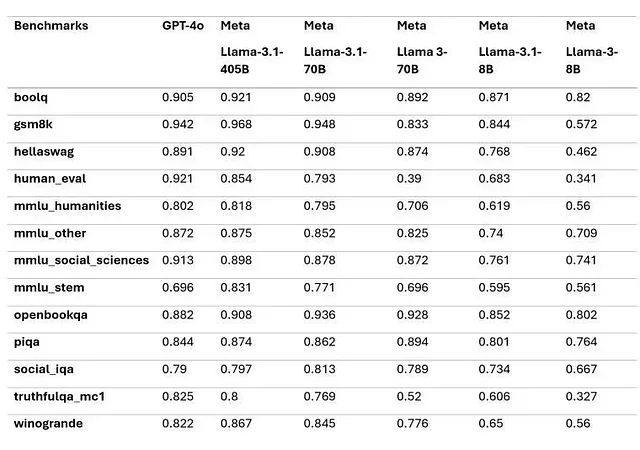
\includegraphics[width=0.8\textwidth]{medium_llama-gpt.png}
    \caption[13F voorbeeld 4]{\label{fig:gpt-vs-llama-benchmarks} Afbeeldingtoont een statistische vergelijking van GPT- en LLaMA-modellen op veelgebruikte NLP-benchmarks.}
\end{figure}
 
\paragraph{Conclusie}

Samengevat is GPT een geavanceerde, commercieel verkrijgbare optie voor sommige NLP-taken, terwijl LLaMA een praktisch open-source alternatief is, vooral wanneer financiële beperkingen of de behoefte aan personalisatie van het grootste belang zijn. Door een zorgvuldige selectie, training en fijnafstemming van LLaMA-modellen is het mogelijk om betrouwbare resultaten te verkrijgen die op maat zijn gemaakt voor gerichte toepassingen, zonder de kosten te hoeven maken die gepaard gaan met aangeschafte modellen zoals GPT.












% ----------------------------------------------------------------------------
\section{Technieken en Tools}
\subsection{SpaCy vs NLTK}
De volgende tabel geeft een vergelijkende analyse van SpaCy en NLTK op basis van belangrijke functies die relevant zijn voor tekstsamenvatting.

\autocite{amade2024automatic}
\begin{table}[h!]
    \centering
    \begin{tabular}{|p{4cm}|p{5cm}|p{5cm}|}
        \hline
        \textbf{Functie} & \textbf{NLTK} & \textbf{SpaCy} \\ \hline
        \textbf{Precisie} & 0.51 & 0.72 \\ \hline
        \textbf{Recall} & 0.65 & 0.65 \\ \hline
        \textbf{F-Score} & 0.58 & 0.69 \\ \hline
        \textbf{Tokenisatiesnelheid} & 4 ms & 0.2 ms \\ \hline
        \textbf{Taggingsnelheid} & 443 ms & 1 ms \\ \hline
        \textbf{Ondersteuning voor Classificatie} & Ja & Ja \\ \hline
        \textbf{Onderwerpmodellering} & Nee & Ja \\ \hline
        \textbf{Vectorisatie} & Nee & Ja \\ \hline
        \textbf{Parsing} & Ja & Ja \\ \hline
        \textbf{TF-IDF Implementatie} & Nee & Ja \\ \hline
        \textbf{Programmeerparadigma} & Procedureel & Objectgeoriënteerd \\ \hline
        \textbf{Gebruiksvriendelijkheid} & Vereist meer aanpassing en tijd & Meer geautomatiseerd en gebruiksvriendelijk \\ \hline
        \textbf{Ondersteunde Taalmodellen} & Basis Tokenizatie en parsing & Geavanceerde modellen met voorgetrainde vectors \\ \hline
        \textbf{Grootte en Afhankelijkheden van de Bibliotheek} & Lichtgewicht, minimale afhankelijkheden & Zwaarder, meer afhankelijkheden door geavanceerde functies \\ \hline
    \end{tabular}
    \caption{Vergelijkende Analyse van SpaCy en NLTK}
    \label{tab:comparison}
\end{table}


\textbf{Prestatiewaarden (Precisie, Recall, F-Score):} SpaCy toont hogere precisie (0.72 vs. 0.51) en F-Score (0.69 vs. 0.58) in vergelijking met NLTK, wat wijst op superieure nauwkeurigheid bij het genereren van samenvattingen.

\textbf{Snelheid van Tokenizatie en Tagging:} SpaCy is aanzienlijk sneller dan NLTK in zowel tokeniseren als taggen. SpaCy kan bijvoorbeeld tekst tokenen in 0,2 milliseconden vergeleken met de 4 milliseconden van NLTK, waardoor het geschikter is voor toepassingen die real-time verwerking vereisen.
\textbf{Ondersteuning voor Geavanceerde NLP-functies:} SpaCy ondersteunt geavanceerde functies zoals topic modellering, vectorisatie en TF-IDF (Term Frequency-Inverse Document Frequency), die niet standaard beschikbaar zijn in NLTK. Dit maakt SpaCy een meer uitgebreide tool voor taken die diep semantisch begrip en machine learning integratie vereisen.

\textbf{Gebruiksvriendelijkheid:} SpaCy is gebruiksvriendelijker met ingebouwde mogelijkheden, wat de behoefte aan maatwerkprogrammering vermindert, in tegenstelling tot NLTK, dat meer tijd en inspanning vergt.

\paragraph{subsubsection}{Conclusie}
Samenvattend, SpaCy is een krachtigere en efficiëntere tool voor tekstsamenvatting vanwege zijn hogere precisie, snelheid en ondersteuning voor geavanceerde NLP-functies. NLTK, hoewel veelzijdig, is beter geschikt voor eenvoudigere taken of projecten die meer aanpassing vereisen. De keuze tussen deze tools hangt af van de specifieke eisen van het project, waaronder de complexiteit van de taak, de benodigde functies en de beschikbare middelen.


\subsection{Database Management Systemen (DBMS)}
In deze sectie gaan wij bekijken welke databank gebruikt zal worden na het structuren en standaardiseren van de 13f meldingen. Hier zal besproken worden of er SQL of nosql gebruikt zal worden vervolgens zal er een specifieke databank gekozen worden
\subsubsection{SQL vs. NOSQL}
Bij het kiezen tussen SQL- en Nosql-databases is het belangrijk om de onderliggende architectuur en toepassingsmogelijkheden te begrijpen. SQL-databases zijn ontworpen voor het organiseren van gestructureerde data, waardoor ze ideaal zijn voor online transaction processing (OLTP). Ze presteren uitstekend in situaties waarin complexe query’s, consistentie en relationeel databeheer vereist zijn. Nosql-databases daarentegen ondersteunen horizontale schaalbaarheid en zijn geoptimaliseerd voor het verwerken van grote hoeveelheden ongestructureerde data, wat hen geschikt maakt voor big data-analyse. De keuze tussen beide hangt grotendeels af van de specifieke behoeften van de organisatie, zoals de focus op datastructuur of schaalbaarheid \autocite{khan2023performance}.

In dit onderzoek is gekozen voor een SQL-database. Deze keuze is gebaseerd op de noodzaak om gestructureerde data uit de 13F-meldingen te beheren, waarbij consistente gegevensintegriteit en de mogelijkheid om complexe query’s uit te voeren cruciaal zijn. SQL-databases bieden de benodigde functionaliteiten voor het beheer van relationele gegevens en het uitvoeren van geavanceerde analyses, wat essentieel is voor het succes van dit project \autocite{khan2023performance}.

\paragraph{SQL-databank}
Op basis van de gedetailleerde analyse die door \autocite{Javija2024} werd PostgreSQL gekozen voor ons proefschrift vanwege de geavanceerde functies, robuuste gegevensintegriteit en uitbreidbare architectuur. In tegenstelling tot andere SQL-databases, blinkt PostgreSQL uit in het verwerken van complexe datamanipulatie, het bieden van sterke ACID compliance en het ondersteunen van aangepaste datatypes en functies. Dit maakt PostgreSQL bijzonder geschikt voor bedrijfstoepassingen en datawarehousing waar schaalbaarheid en geavanceerd databeheer cruciaal zijn. Hoewel PostgreSQL een steilere leercurve heeft dan sommige alternatieven, maken de uitgebreide functie set en betrouwbaarheid het een optimale keuze om aan de complexe eisen van ons project te voldoen.


% ----------------------------------------------------------------------------

\section{Uitdagingen en beperkingen}
In dit hoofdstuk zullen enkele uitdagingen en beperkingen benoemt worden
\subsection{Variable structuur}
Vóór 2013 bevatten 13F-meldingen enigszins verschillende variabele structuren, maar deze variaties zijn belangrijk omdat ze het moeilijk maken om de gegevens te lezen en te analyseren. Vóór 2013 waren de 13F-meldingen variabeler in de manier waarop ze gegevens verstrekten, waardoor het moeilijk was om beleggingsportefeuilles door de tijd heen te vergelijken. Door dit gebrek aan standaardisatie moesten onderzoekers en analisten zorgvuldig omgaan met deze gegevens om consistente en nauwkeurige bevindingen te krijgen. Diepgaand onderzoek is nodig om interpretatiefouten te minimaliseren en investeringen en investeringspatronen als gevolg van verschillende rapportagestandaarden volledig te begrijpen.
\subsection{Gegevenskwaliteit en Validatie}
Het valideren van grote taalmodellen (LLM's) brengt verschillende uitdagingen met zich mee:

\begin{itemize}
    \item \textbf{Complexiteit van metrieken}: Geen enkele metriek omvat alle prestatieaspecten en het combineren van metrieken kan leiden tot inconsistenties.
    \item \textbf{Contextgevoeligheid}: Modelprestaties variëren met de context, wat de evaluatie bemoeilijkt.
    \item \textbf{Subjectiviteit}: Menselijke evaluaties zijn subjectief en kunnen variëren tussen verschillende personen.
    \item \textbf{Rekenkracht}: Uitgebreide validatie vereist aanzienlijke rekenkracht.
    \item  \textbf{Dynamische industrie} Met de snelle vooruitgang in NLP kunnen validatiemethoden snel verouderen.
\end{itemize}



\subsection{Databaseprestaties}
Uitdaging: Hoewel PostgreSQL goed presteert bij grote hoeveelheden gestructureerde data, kan het moeilijk zijn om de prestaties te optimaliseren naarmate de hoeveelheid data en het aantal gelijktijdige gebruikers toeneemt.

Beperking: Bij zeer grote datasets of een hoge mate van gelijktijdige toegang kunnen er prestatieproblemen optreden. Het kan nodig zijn om uitgebreide optimalisaties en schaalstrategieën te implementeren, zoals partitionering of het gebruik van read replicas.
% ----------------------------------------------------------------------------
\section{Tekortkomingen in huidig onderzoek}
Dit hoofdstuk geeft enkele gaten weer in het huidig onderzoek.
\subsection{Onbehandelde kwesties}
\paragraph{Training van Eigen Large Language Models (LLMs)}
Het trainen van een eigen LLM voor financiële toepassingen vereist veel tijd en middelen. Het model moet worden getraind op uitgebreide financiële datasets voor nauwkeurige resultaten. Dit kan uw infrastructuur belasten en vereist expertise in machine learning en datawetenschap, met mogelijke problemen op het gebied van data-integriteit en privacy.

\paragraph{Beveiliging en Privacy}
Het beschermen van gevoelige financiële gegevens tegen ongeautoriseerde toegang en datalekken is complex en vereist naleving van privacywetgeving. Onvoldoende beveiliging kan leiden tot datalekken, verlies van vertrouwen en juridische problemen. Implementeer encryptie, toegangscontrole en regelmatige beveiligingsaudits om gegevens te beschermen. Zorg ervoor dat uw systemen voldoen aan relevante regelgeving en best practices voor gegevensbeveiliging.

\paragraph{Schaalbaarheid en Prestaties}
Groeiende hoeveelheden gegevens kunnen leiden tot prestatieproblemen bij opslag en analyse, wat complexe oplossingen vereist voor snelle toegang. Slechte prestaties kunnen vertragingen veroorzaken in rapportage en analyse, wat de besluitvorming en efficiëntie beïnvloedt. Gebruik schaalbare databases en technieken zoals gegevenspartitionering en caching. Monitor en optimaliseer regelmatig de prestaties om problemen te voorkomen.
